\subsubsection{Example}

    \begin{itemize}[noitemsep,topsep=0pt]
      \item Starting position: (63.0, -58.0, 102.0)
      \item End position: (-1.0, -1.0, 9.0) 
      \item Euclidean distance from the object: 9.1104335791443
      \item Object can be seen: True
      \item Success: True
      \item Object type: road construction site
      
    \end{itemize}
    

    \begin{center}
    \includegraphics[width=0.7\linewidth]{images/Sonnet-CityNew-FS2/34.pdf}
    \end{center}
    

    \begin{center}
    \includegraphics[width=0.7\linewidth]{images/Sonnet-CityNew-FS2/34_sit_awareness.pdf}
    \end{center}
    

    \begin{drama}
    \Character{Benchmark}{re}
    \Character{Claude 3.5 Sonnet}{gpt}
    
\respeaks: \( < \)Context\( > \)
    You are in command of a UAV, tasked with finding road construction site.
\( < \)/Context\( > \) \texttt{(REST OF THE PROMPT)}
\respeaks: The object you're looking for is similar to this. This is NOT the drone's current view.
\respeaks: Image 1:
\StageDir{\re{} presents \gpt{} with a relevant image}

    \begin{center}
    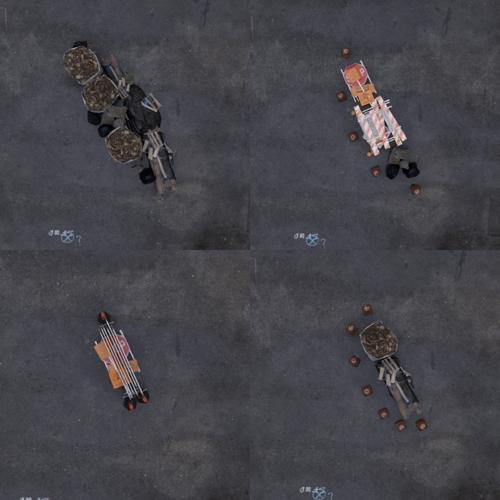
\includegraphics[width=0.5\linewidth]{images/Sonnet-CityNew-FS2/34_0.jpg}
    \end{center}
    
\respeaks: Your current altitude is 102 meters above ground level.
\respeaks: Image 2:
\StageDir{\re{} presents \gpt{} with a relevant image}

    \begin{center}
    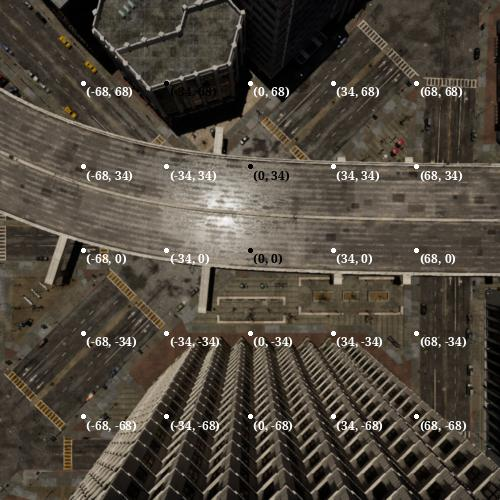
\includegraphics[width=0.5\linewidth]{images/Sonnet-CityNew-FS2/34_1.jpg}
    \end{center}
    
\gptspeaks: \( < \)Reasoning\( > \)I can see a wide urban area from my current position at 102 meters. Given that I'm looking for road construction equipment similar to what was shown in the reference image, I need to get lower to better identify potential targets. I notice some construction-like activity near the coordinates (-34, -34). I'll move there and decrease altitude significantly to get a better view.\( < \)/Reasoning\( > \)
\( < \)Action\( > \)(-34, -34, -70)\( < \)/Action\( > \)
\respeaks: Your current altitude is 32 meters above ground level.
\respeaks: Image 3:
\StageDir{\re{} presents \gpt{} with a relevant image}

    \begin{center}
    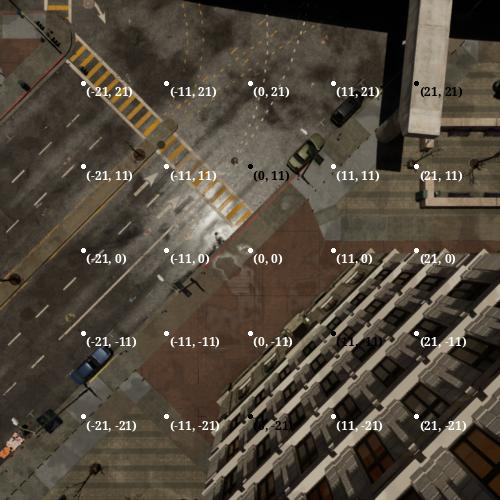
\includegraphics[width=0.5\linewidth]{images/Sonnet-CityNew-FS2/34_2.jpg}
    \end{center}
    
\gptspeaks: \( < \)Reasoning\( > \)I can see some construction-related activity in this area, but I need to get closer to confirm. I notice something that might be construction equipment near (-11, 11). I'll move there and decrease altitude to get under 10 meters for a better view.\( < \)/Reasoning\( > \)
\( < \)Action\( > \)(-11, 11, -23)\( < \)/Action\( > \)
\respeaks: Your current altitude is 9 meters above ground level.
\respeaks: Image 4:
\StageDir{\re{} presents \gpt{} with a relevant image}

    \begin{center}
    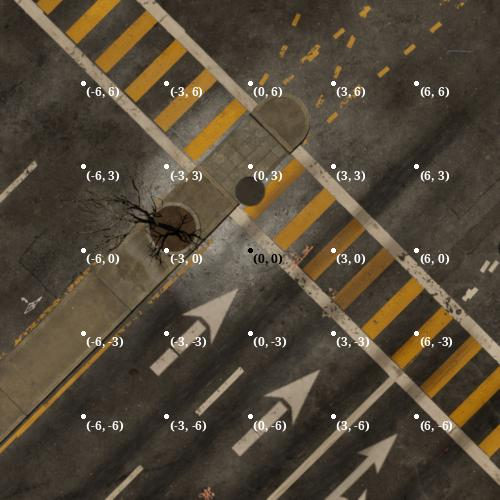
\includegraphics[width=0.5\linewidth]{images/Sonnet-CityNew-FS2/34_3.jpg}
    \end{center}
    
\gptspeaks: \( < \)Reasoning\( > \)From this position, I can see road markings and some construction work, but I don't see the specific type of construction equipment I'm looking for (like what was shown in the reference image). I'll move towards (3, 6) where I can see some yellow markings that might be related to construction activity.\( < \)/Reasoning\( > \)
\( < \)Action\( > \)(3, 6, 0)\( < \)/Action\( > \)
\respeaks: Your current altitude is 9 meters above ground level.
\respeaks: Image 5:
\StageDir{\re{} presents \gpt{} with a relevant image}

    \begin{center}
    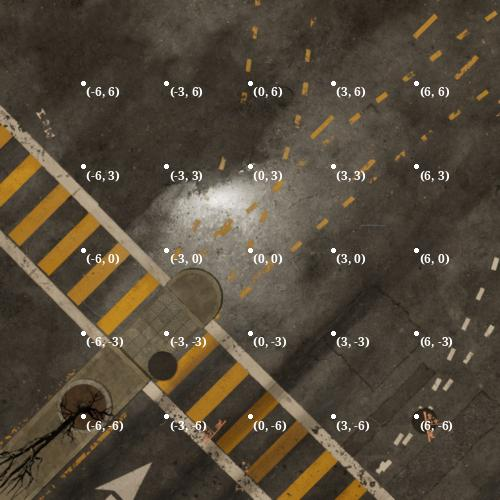
\includegraphics[width=0.5\linewidth]{images/Sonnet-CityNew-FS2/34_4.jpg}
    \end{center}
    
\gptspeaks: \( < \)Reasoning\( > \)I still don't see the specific construction equipment I'm looking for in this area. I need to explore more of the search area. I'll move towards (-6, 3) to check the area with some different markings on the road.\( < \)/Reasoning\( > \)
\( < \)Action\( > \)(-6, 3, 0)\( < \)/Action\( > \)
\respeaks: Your current altitude is 9 meters above ground level.
\respeaks: Image 6:
\StageDir{\re{} presents \gpt{} with a relevant image}

    \begin{center}
    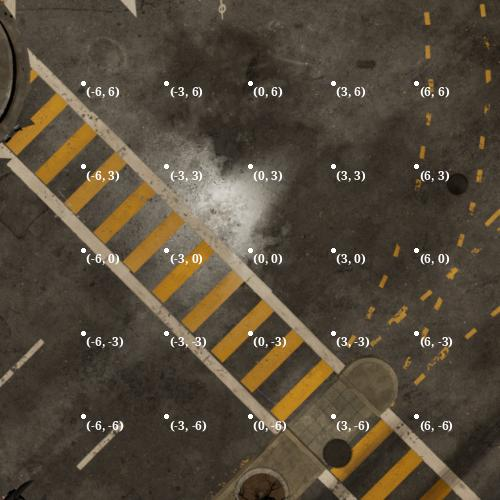
\includegraphics[width=0.5\linewidth]{images/Sonnet-CityNew-FS2/34_5.jpg}
    \end{center}
    
\gptspeaks: \( < \)Reasoning\( > \)The construction equipment isn't visible in this section either. I need to explore more of the initial search area. Let's move back to a different section where there might be construction activity. I'll head towards (-21, 0) to check another part of the road.\( < \)/Reasoning\( > \)
\( < \)Action\( > \)(-21, 0, 0)\( < \)/Action\( > \)
\respeaks: Your current altitude is 9 meters above ground level.
\respeaks: Image 7:
\StageDir{\re{} presents \gpt{} with a relevant image}

    \begin{center}
    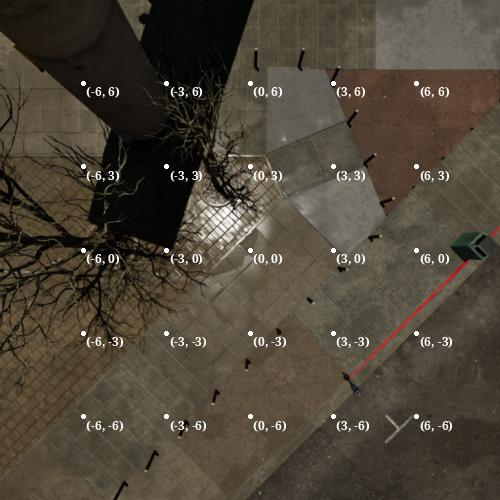
\includegraphics[width=0.5\linewidth]{images/Sonnet-CityNew-FS2/34_6.jpg}
    \end{center}
    
\gptspeaks: \( < \)Reasoning\( > \)This area shows different pavement patterns but no construction equipment. I need to check another section of the search area. I'll move towards (11, -11) to investigate an area we haven't explored yet.\( < \)/Reasoning\( > \)
\( < \)Action\( > \)(11, -11, 0)\( < \)/Action\( > \)
\respeaks: Your current altitude is 9 meters above ground level.
\respeaks: Image 8:
\StageDir{\re{} presents \gpt{} with a relevant image}

    \begin{center}
    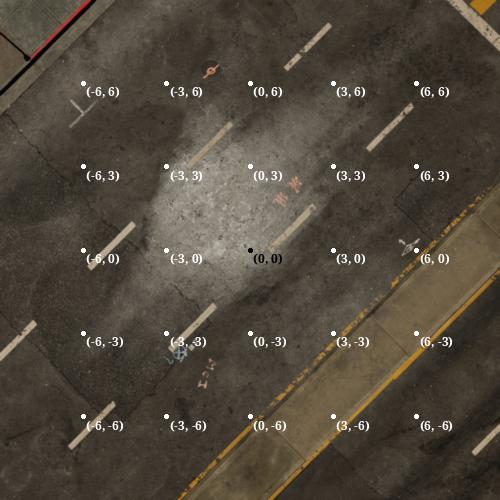
\includegraphics[width=0.5\linewidth]{images/Sonnet-CityNew-FS2/34_7.jpg}
    \end{center}
    
\gptspeaks: \( < \)Reasoning\( > \)Still no sign of the construction equipment we're looking for. Let's check the area near (34, -34) where there might be more construction activity. We haven't explored that section yet.\( < \)/Reasoning\( > \)
\( < \)Action\( > \)(34, -34, 0)\( < \)/Action\( > \)
\respeaks: Emergency stop; you've flown too close to something and would have hit it.
\respeaks: Your current altitude is 9 meters above ground level.
\respeaks: Image 9:
\StageDir{\re{} presents \gpt{} with a relevant image}

    \begin{center}
    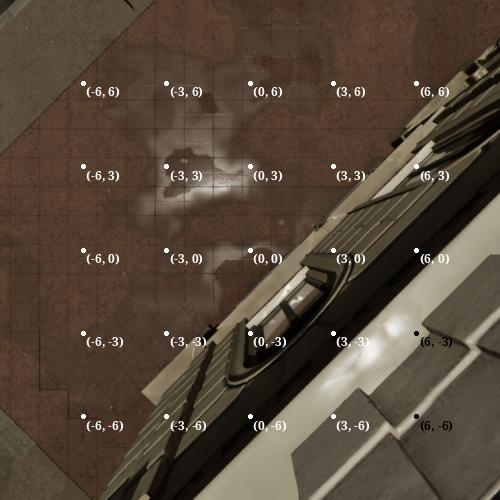
\includegraphics[width=0.5\linewidth]{images/Sonnet-CityNew-FS2/34_8.jpg}
    \end{center}
    
\gptspeaks: \( < \)Reasoning\( > \)I apologize for the unsafe move. I need to be more careful about obstacles. Let's move to a safer location and continue our search. I'll head towards (-34, 0) where there appears to be more open space.\( < \)/Reasoning\( > \)
\( < \)Action\( > \)(-34, 0, 0)\( < \)/Action\( > \)
\respeaks: Your current altitude is 9 meters above ground level.
\respeaks: Image 10:
\StageDir{\re{} presents \gpt{} with a relevant image}

    \begin{center}
    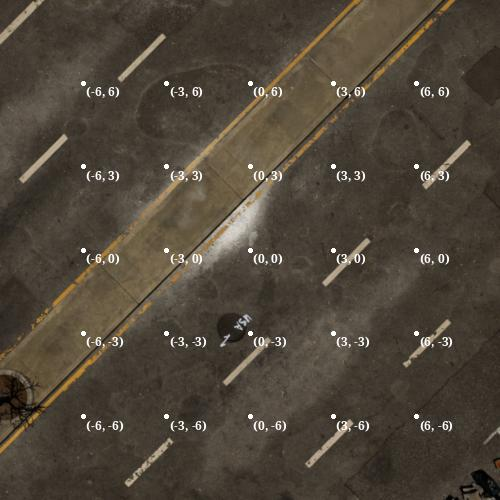
\includegraphics[width=0.5\linewidth]{images/Sonnet-CityNew-FS2/34_9.jpg}
    \end{center}
    
\gptspeaks: \( < \)Reasoning\( > \)I see something that looks like construction equipment at coordinates (0, -3). Let me center on it to confirm if it matches what we're looking for.\( < \)/Reasoning\( > \)
\( < \)Action\( > \)(0, -3, 0)\( < \)/Action\( > \)
\respeaks: Your current altitude is 9 meters above ground level.
\respeaks: Image 11:
\StageDir{\re{} presents \gpt{} with a relevant image}

    \begin{center}
    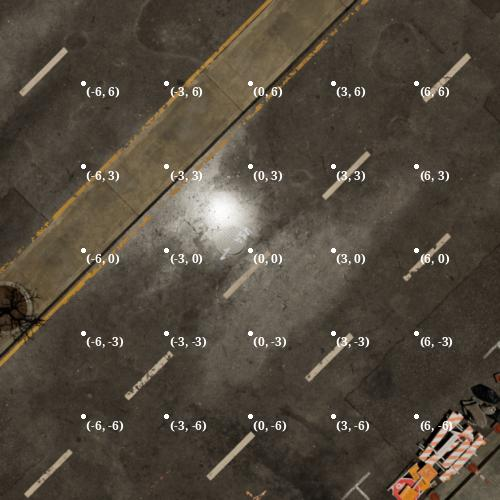
\includegraphics[width=0.5\linewidth]{images/Sonnet-CityNew-FS2/34_10.jpg}
    \end{center}
    
\gptspeaks: \( < \)Reasoning\( > \)I can see what appears to be road construction equipment in the lower right corner of the image, matching the reference image shown earlier. Let me move closer to it at coordinates (6, -6) to confirm.\( < \)/Reasoning\( > \)
\( < \)Action\( > \)(6, -6, 0)\( < \)/Action\( > \)
\respeaks: Your current altitude is 9 meters above ground level.
\respeaks: Image 12:
\StageDir{\re{} presents \gpt{} with a relevant image}

    \begin{center}
    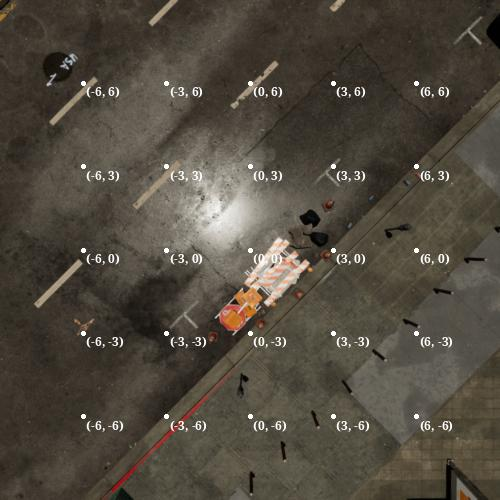
\includegraphics[width=0.5\linewidth]{images/Sonnet-CityNew-FS2/34_11.jpg}
    \end{center}
    
\gptspeaks: FOUND
\end{drama}
\subsubsection{Example}

    \begin{itemize}[noitemsep,topsep=0pt]
      \item Starting position: (31.0, 8.0, 108.0)
      \item End position: (1.0, -2.0, 9.0) 
      \item Euclidean distance from the object: 9.273618495495704
      \item Object can be seen: True
      \item Success: True
      \item Object type: fire
      
    \end{itemize}
    

    \begin{center}
    \includegraphics[width=0.7\linewidth]{images/Sonnet-CityNew-FS2/39.pdf}
    \end{center}
    

    \begin{center}
    \includegraphics[width=0.7\linewidth]{images/Sonnet-CityNew-FS2/39_sit_awareness.pdf}
    \end{center}
    

    \begin{drama}
    \Character{Benchmark}{re}
    \Character{Claude 3.5 Sonnet}{gpt}
    
\respeaks: \( < \)Context\( > \)
    You are in command of a UAV, tasked with finding fire.
\( < \)/Context\( > \) \texttt{(REST OF THE PROMPT)}
\respeaks: The object you're looking for is similar to this. This is NOT the drone's current view.
\respeaks: Image 1:
\StageDir{\re{} presents \gpt{} with a relevant image}

    \begin{center}
    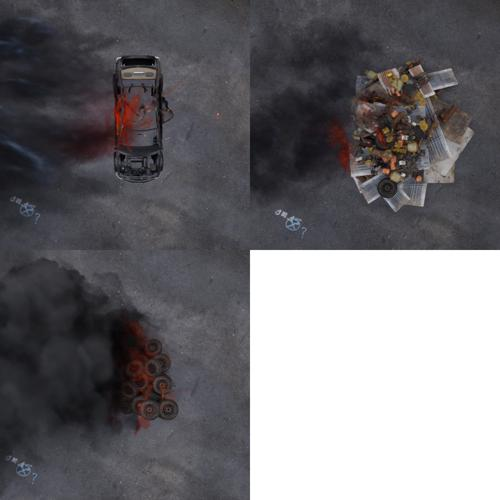
\includegraphics[width=0.5\linewidth]{images/Sonnet-CityNew-FS2/39_0.jpg}
    \end{center}
    
\respeaks: Your current altitude is 108 meters above ground level.
\respeaks: Image 2:
\StageDir{\re{} presents \gpt{} with a relevant image}

    \begin{center}
    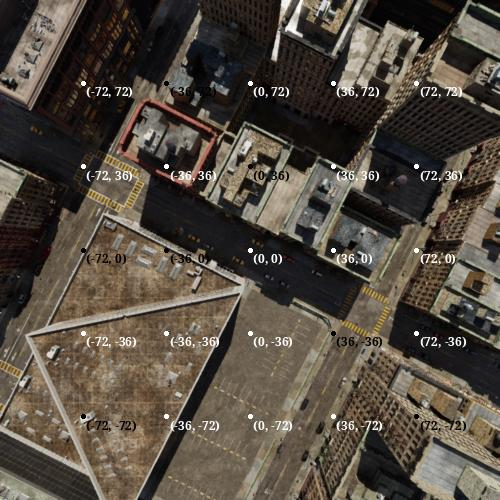
\includegraphics[width=0.5\linewidth]{images/Sonnet-CityNew-FS2/39_1.jpg}
    \end{center}
    
\gptspeaks: \( < \)Reasoning\( > \)
I need to start a systematic search for any signs of fire. Given the example images show objects on fire at ground level, I should begin by lowering my altitude to get a better view while maintaining a safe height initially. I'll start by moving to the center of the visible area (0,0) and descending to about 50 meters to get a better overview while still maintaining good visibility.
\( < \)/Reasoning\( > \)
\( < \)Action\( > \)(0, 0, -58)\( < \)/Action\( > \)
\respeaks: Your current altitude is 50 meters above ground level.
\respeaks: Image 3:
\StageDir{\re{} presents \gpt{} with a relevant image}

    \begin{center}
    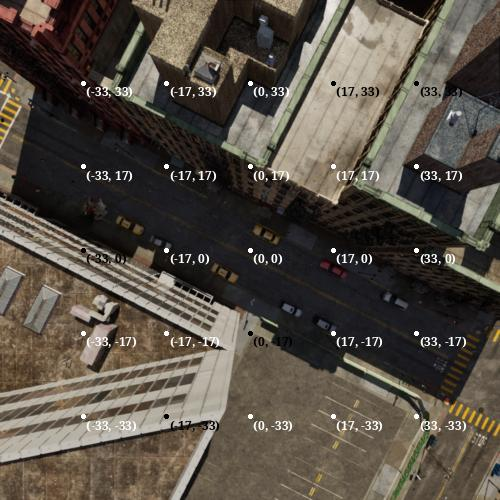
\includegraphics[width=0.5\linewidth]{images/Sonnet-CityNew-FS2/39_2.jpg}
    \end{center}
    
\gptspeaks: \( < \)Reasoning\( > \)
From this lower altitude, I can see more detail. I notice what appears to be some objects on the street around (-17, 0). I should move closer to that area and descend further to get a better look at what might be potential fire hazards or burning objects.
\( < \)/Reasoning\( > \)
\( < \)Action\( > \)(-17, 0, -35)\( < \)/Action\( > \)
\respeaks: Your current altitude is 15 meters above ground level.
\respeaks: Image 4:
\StageDir{\re{} presents \gpt{} with a relevant image}

    \begin{center}
    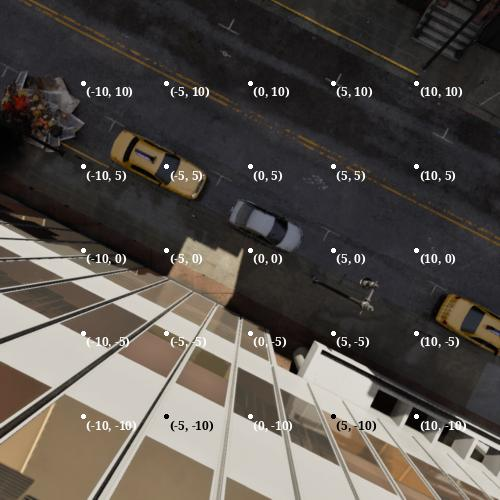
\includegraphics[width=0.5\linewidth]{images/Sonnet-CityNew-FS2/39_3.jpg}
    \end{center}
    
\gptspeaks: \( < \)Reasoning\( > \)
I can see what appears to be flames or fire at approximately (-10, 10). I should move directly over it and descend slightly to get within 10 meters while keeping it in my field of view.
\( < \)/Reasoning\( > \)
\( < \)Action\( > \)(-10, 10, -6)\( < \)/Action\( > \)
\respeaks: Your current altitude is 9 meters above ground level.
\respeaks: Image 5:
\StageDir{\re{} presents \gpt{} with a relevant image}

    \begin{center}
    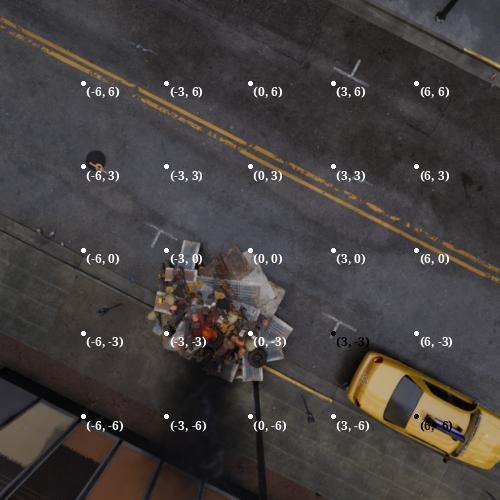
\includegraphics[width=0.5\linewidth]{images/Sonnet-CityNew-FS2/39_4.jpg}
    \end{center}
    
\gptspeaks: \( < \)Reasoning\( > \)
I can now clearly see the burning debris/fire at my current position. I am at 9 meters altitude which is below the required 10 meters, and the fire is directly in my field of view. I am properly centered over the target.
\( < \)/Reasoning\( > \)
FOUND
\end{drama}
